\input{../Preambulos/preambulo_materiales}
\usetikzlibrary{decorations.text}
\usetikzlibrary{patterns, arrows}
\usetikzlibrary{decorations.pathmorphing, decorations.markings}
\usetikzlibrary{matrix}

% \documentclass[letterpaper]{article}
% \usepackage[utf8]{inputenc}
% %\usepackage[latin1]{inputenc}
% \usepackage[spanish]{babel}
% \usepackage{geometry}
% \usepackage{anysize}
% \usepackage{graphicx} 
% \usepackage{amsmath}
% \usepackage{tikz}
% % \usetikzlibrary{patterns}

% \usetikzlibrary{decorations.pathmorphing,patterns}
% \usetikzlibrary{decorations.markings}
% \usetikzlibrary{matrix}
% \usepackage{xy}
% \usepackage{siunitx}
% \usepackage[american,cuteinductors,smartlabels]{circuitikz}
% \usetikzlibrary{calc}
% \usepackage{color}
% %\numberwithin{equation}{list}
% \marginsize{1cm}{2cm}{0cm}{2cm}  

\title{Ejericicios del Examen Tema 3 \\ {\large Curso Física Computacional}}
\author{M. en C. Gustavo Contreras Mayén. \texttt{gux7avo@ciencias.unam.mx}}

\date{ }
\begin{document}

\maketitle
\fontsize{14}{14}\selectfont

A continuación se presenta la lista de ejercicios a resolver que conforman la parte de la evaluación del Tema 3, recuerda que el segundo examen parcial corresponde a los Temas 3 y 4, con la finalidad de brindar más tiempo en la solución de los problemas, se entrega anticipadamente la lista de ejercicios.
\par
Cada ejercicio tiene una calificación de un punto siempre y cuando esté debidamente resuelto, se ocupará la rúbrica de evaluación que ya conoces.
\par
Revisa cuidadosamente cada ejercicio, ya que deberás de mencionar qué técnica de solución has elegido y justificar su uso, en caso de que el problema indique expresamente la técnica a utilizar, no será necesario que lo expliques.

\begin{enumerate}
\item Un depósito cónico contiene agua hasta $\SI{0.5}{\meter}$ de altura a partir del fondo. El depósito tiene un orificio en el fondo, de $\SI{0.02}{\meter}$ de radio. El radio del depósito está dado por $r = 0.25 \, y$, donde $r$ es el radio y $y$ la altura medida desde el fondo. La velocidad del agua que pasa por el orificio está dada por $v^{2} = 2 \, g \, y$. Con el método de Euler ($h = 0.001$), calcula cuántos minutos se tardará en vaciar el depósito.
\item Un tanque de $50$ galones de agua contiene sal con una concentración de $10$ onzas/galón. Con el fin de diluir el contenido de sal, se suministra agua pura a razón de $2$ galones/minuto.
\begin{enumerate}
\item Si el depósito tiene una mezcla uniforme y la misma cantidad de agua que entra sale del depósito cada minuto, la concentración de sal satisface:
\begin{align*}
\pderivada{y}_{1} (t) = - \dfrac{2}{50} \, y_{1}, \hspace{1.5cm} y_{1} (0) = 10
\end{align*}
donde $y_{1} (t)$ es la concentración de sal en onzas/galón y $t$ es el tiempo en minutos. Usando el método de RK2 y $h = 1$ minuto, calcula cuánto tiempo debe de transcurrir para que la concentración de sal sea $1/10$ de su valor inicial.
\item El agua que sale del tanque entra a otro tanque de $20$ galones, en el cual también se vierte agua pura a razón de $3$ galones/minuto y se mezcla bien. La concentración de sal en el segundo tanque satisface:
\begin{align*}
\pderivada{y}_{2} (t)= - \dfrac{3}{20} \, y_{2} (t)+ \dfrac{2}{20} \, y_{1} (t), \hspace{1.5cm} y_{2}(0) = 0
\end{align*}
donde $y_{1} (t)$ es la concentración de sal del tanque de $50$ galones del inciso anterior. Usando RK2, determina cuándo alcanza su máximo de concentración de sal en el tanque de $20$ galones. Supongamos que el segundo tanque tiene agua pura en $t = 0$.
\end{enumerate}
% Ref. Kiusaalas (2005) 7.3 RK Methods
% Problema 11
\item Un péndulo está suspendido en un collar deslizante. El sistema está en reposo, posteriormente se aplica al collar un movimiento oscilante: $y (t) = Y \, \sin \omega t$, en $t = 0$. La ecuación diferencial que describe el movimiento del péndulo es:
\begin{align*}
\ddot{\theta} = - \dfrac{g}{L} \sin \theta + \dfrac{\omega^{2}}{L} Y \, \cos \theta \, \sin \omega t
\end{align*}
\begin{figure}[H]
\centering
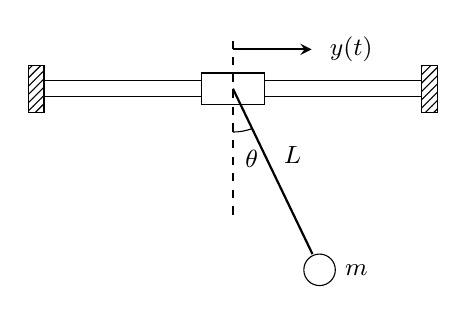
\begin{tikzpicture}[font=\small]
	\draw (-0.1,-0.2) [pattern = north east lines] rectangle (0.1,0.4);
	\draw (4.9,-0.2) [pattern = north east lines] rectangle (5.1,0.4);
	\draw (0.1,0.0) rectangle (4.9,0.2);
	\draw (2.1,-0.1) [fill=white] rectangle (2.9,0.3);
	\draw [dashed] (2.5,-1.5) -- (2.5,0.7);
	\draw [-stealth, thick] (2.5,0.6) -- node [right=0.6cm] {$y (t)$} (3.5,0.6);
	\draw [thick] (2.5,0.1) -- node [near end, above=0.5cm]{$L$}(3.51,-2.);
	\draw (3.6,-2.2) circle (0.2) node [right=0.2cm] {$m$};
	\draw (2.5,-0.45) arc (270:290:7mm) node [below=0.15cm]{$\theta$};
\end{tikzpicture}
\end{figure}
Grafica $\theta$ contra $t$ en el intervalo de $t = 0$ a $t = 10$ segundos, así mismo, determina el desplazamiento mayor de $\theta$ durante éste período. Usa $g = \SI{9.80665}{\meter\per\square\second}$, $L = \SI{1.0}{\meter}$, $Y = \SI{0.25}{\meter}$ y $\omega = \SI{2.5}{\radian\per\second}$.
% Ref. Kiusaalas (2013) 7.3 RK Methods
% Problema 12
\item Tenemos un sistema que consiste en un masa que se desliza sobre una barra guía que está en reposo, la masa se ubica en $r = \SI{0.75}{\meter}$. Al tiempo $t = 0$ se enciende un motor que proporiona un movimiento dado por la expresión $\theta (t) = (\pi/12) \cos \pi t$ sobre la barra. La EDO que describe el movimiento resultante de la masa deslizante es:
\begin{align*}
\ddot{r} = \left( \dfrac{\pi^{2}}{12}\right)^{2}  r \sin^{2} \pi t - g \sin \left( \dfrac{\pi}{12} \cos \pi t \right)
\end{align*}
\begin{figure}[H]
\centering
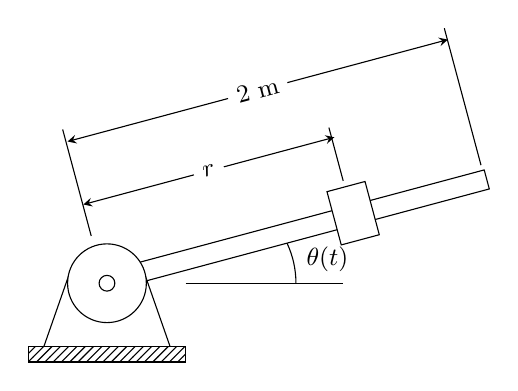
\begin{tikzpicture}[font=\small]
	\draw (0,0) [pattern = north east lines] rectangle (2,0.2);
	\draw (0.2,0.2) -- (0.55,1.2);
	\draw (1.8,0.2) -- (1.45,1.2);
	\draw (0.9,0.9) [rotate around={15:(1,1)}]rectangle (6,1.15);
	\draw (1,1) [fill=white] circle (0.5);
	\draw (1,1) circle (0.1);
	\draw (4,0.7) [fill=white, rotate around={15:(1,1)}]rectangle (4.5,1.4);
	\draw (2,1) -- (4,1);
	\draw (3.4,1) arc (0:25:12mm);
	\draw (3.8,1.3) node {$\theta(t)$};
	\draw (0.8,1.6) [rotate around={15:(0.8,1.6)}] -- (0.8,3);
	\draw (4,2.3) [rotate around={15:(4,2.3)}] -- (4,3);
	\draw (5.75,2.5) [rotate around={15:(5.75,2.5)}] -- (5.75,4.3);
	\draw [stealth-stealth, rotate around={15:(0.7,2)}] (0.7,2)  -- node [rotate=15,midway, fill=white]{$r$}(4,2);
	\draw [stealth-stealth, rotate around={15:(0.5,2.8)}] (0.5,2.8)  -- node [rotate=15,midway, fill=white]{$2 \mbox{ m}$}(5.5,2.8);
	\end{tikzpicture}
\end{figure}
Calcula el tiempo para el cual, la masa deslizante alcanza el extremo final de la barra guía (la punta de la barra). Usa el valor de $g = \SI{9.80665}{\meter\per\square\second}$.
% Problema 13
\item Una bala de masa $m = \SI{0.25}{\kilo\gram}$ se lanza con una velocidad $v_{0} = \SI{50}{\meter\per\second}$ en la dirección que se indica en la siguiente figura.
\begin{figure}[H]
\centering
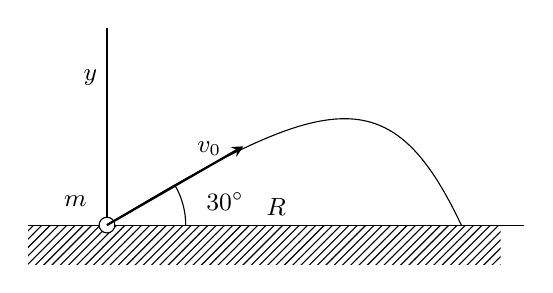
\begin{tikzpicture}[font=\small]
	\draw (0,0) [pattern = north east lines, draw = none] rectangle (6,0.5);
	\draw (0,0.5) -- node [midway, above] {$R$} (6.3,0.5);
	\draw (1,0.5) -- node [near end, left] {$y$} (1,3);
	\draw [fill=white] (1,0.5) circle (0.1);
	\draw (0.6,0.8) node {$m$};
	\draw [-stealth, rotate around={30:(1,0.5)}, thick] (1,0.5) -- node [near end, above] {$v_{0}$} (3,0.5);
	\draw (2,0.5) arc (0:30:10mm);
	\draw (2.5,0.8) node {$30^{\circ}$};
	\draw (1,0.5) .. controls (3.8,2.2) and (4.6,2.4) .. (5.5,0.5);
%		  (4,2) .. controls (3.9,1.9).. and (4.1,2.1)..(5.5,0.5);
%		  (3.3,1.4) ..controls (4,1.5) and (4.2,1.3) .. (5.5,0.2);%.. controls (3.8,0.3) and (3.5,0.2) .. (5.5,0);
\end{tikzpicture}
\end{figure}
Si la fuerza aerodinámica de arrastre sobre la bala es $F_{D}= C_{D} \, v^{3/2}$, las ecuaciones diferenciales que describen el movimiento son:
\begin{align*}
\ddot{x} = - \dfrac{C_{D}}{m} \, \dot{x} \, v^{1/2} \hspace{2cm} \ddot{y}= - \dfrac{C_{D}}{m} \, \dot{y} \, v^{1/2} - g
\end{align*}
donde $v = \sqrt{\dot{x}^{2} + \dot{y}^{2}}$, $C_{D} = 0.03 \mbox{ kg/(ms)}^{1/2}$ y $g = \SI{9.80665}{\meter\per\square\second}$.

Calcula el tiempo de vuelo y el alcance $R$.
% Problema 15
\item Una masa $m$ está suspendida de una cuerda elástica con una rigidez de extensión $k$ y una longitud sin deformar $L$. 
\begin{figure}[H]
\centering
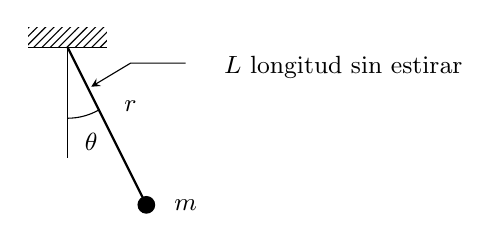
\begin{tikzpicture}[font=\small]
    \draw (0, 0) [pattern = north east lines, draw = none] rectangle (1, 0.25);
    \draw (0, 0) -- (1, 0);
    \draw [thick] (0.5, 0) -- (1.5, -2);
    \node at (1.3, -0.75) {$r$};
    \draw [fill] (1.5, -2) circle (3pt);
    \node at (2, -2) {$m$};
    \draw (0.5, 0) -- (0.5, -1.4);
    \draw (0.5, -0.9) arc(270:300:0.8);
    \node at (0.8, -1.2) {$\theta$};
    \node at (4, -0.25) {$L$ longitud sin estirar};
    \draw [stealth-] (0.8, -0.5) -- (1.3, -0.2) -- (2, -0.2);
\end{tikzpicture}
\end{figure}
\begin{enumerate}
\item Si la masa se suelta desde el reposo en $\theta = \ang{60}$ con la cuerda sin estirar, encuentra la longitud $r$ de la cuerda cuando la posición $\theta = \ang{0}$ se alcanza por primera vez. Las ecuaciones diferenciales que describen el movimiento son:
\begin{align*}
\ddot{r} &= r \, \dot{\theta} + g \, \cos \theta - \dfrac{k}{m} (r - L) \\[0.5em]
\ddot{\theta} &= \dfrac{-2 \, \dot{r} \, \dot{\theta} - g \, \sin \theta}{r}
\end{align*}
Usa $g = \SI{9.80665}{\meter\per\square\second}$, $k = \SI{40}{\newton\per\metre}$ y $m = \SI{0.25}{\kilo\gram}$
\item Resuelve ahora el problema si la masa se libera de la posición $\theta = \ang{60}$ con la cuerda acortada en $\SI{0.075}{\meter}$.
\end{enumerate}
% Problema 19
\item La solución al problema:
\begin{align*}
\sderivada{y} + \dfrac{1}{x} \, \pderivada{y} + y \hspace{1.5cm} y (0) = 1 \hspace{1cm} \pderivada{y}(0) = 0
\end{align*}
es la función de Bessel $J_{0} (x)$. Integra numéricamente para calcular $J_{0} (5)$ y compara el resultado con $-0.17760$, que es el valor que se obtiene de tablas matemáticas. Tip: para evitar la singularidad en $x = 0$, inicia la integración en $x = \num{d-12}$.
% Problema 19
\item Considera el siguiente problema de valores iniciales:
\begin{align*}
\sderivada{y} = 16.81 \, y \hspace{1.5cm} y (0) = 1.0 \hspace{1cm} \pderivada{y} (0) = -4.1
\end{align*}
\begin{enumerate}
\item Obtén la solución analítica.
\item ¿Anticipas dificultades en la solución numérica de este problema?
\item Realiza la integración numérica de $x = 0$ a $8$ para ver si tus preocupaciones estaban justificadas.
\end{enumerate}
% Ref. Kiusaalas 7.5 Adaptive RK method
% Problema 7
\item Calcula la solución numérica de la ED:
\begin{align*}
\sderivada{y} = 16.81 \, y
\end{align*}
de $x = 0$ a $2$ con el método RK Adaptativo y grafica los resultados. Usa las condiciones iniciales:
\begin{enumerate}
\item $y (0) = 1.0$, $\pderivada{y} (0) = -4.1$
\item $y (0) = 1.0$, $\pderivada{y} (0) = -4.11$
\end{enumerate} 
Explica las diferencias en las dos soluciones. Tip: Deriva y gráfica las soluciones analíticas.
% Problema 13
\item Con el método RK Adapativo resuelve:
\begin{align*}
\pderivada{y} = \left( \dfrac{9}{y} - y \right)  \, x \hspace{1.5cm} y (0) = 5
\end{align*}
de $x = 0$ a $4$, grafica $y$ contra $x$.
% Ref. Kiusaalas 8.2 Shooting method
% Problem Set 8.1
% Problema 18
\item Resuelve el problema de CDF:
\begin{align*}
\nderivada{y}{4} = -2 \, y \, \sderivada{y}
\end{align*}
con $y (0) = \pderivada{y} (0) = 0 \hspace{1.5cm} y (4) = 0 \hspace{1cm} \pderivada{y} (4) = 1$.
% Problema 12
\item Resuelve el problema de CDF:
\begin{align*}
\sderivada{y} - \big( 1 - e^{-x} \big) \, y = 0 \hspace{1.5cm} y (0) = 1, \hspace{1cm} y (\infty) = 0
\end{align*}
grafica $y$ contra $x$. Tip: reemplaza el infinito por un valor finito $\beta$. Verifica tu elección de $\beta$ repitiendo la solución con $1.5 \, \beta$. Si los resultados cambian, debes aumentar $\beta$.
% Ref. Kiusaalas 8.3 Finite Differences
% Problem Set 8.2
% Inciso 7
\item Resuelve con el método de diferencias finitas con $m = 20$:
\begin{align*}
\sderivada{y} + 2 \, \pderivada{y} + y = 0, \hspace{1.5cm} y (0) = 0 \hspace{1cm} y (1) = 1
\end{align*}
La solución exacta es $y = x \, e^{1-x}$.
% Inciso 8
\item Resuelve con el método de diferencias finitas con $m = 20$:
\begin{align*}
x^{2} \, \sderivada{y} + x \, \pderivada{y} + y = 0, \hspace{1.5cm} y (1) = 0 \hspace{1cm} y (2) = 0.638961
\end{align*}
La solución exacta es $y = \sin(\ln x)$.
% Inciso 9
\item Resuelve con el método de diferencias finitas con $m = 20$:
\begin{align*}
\sderivada{y} - y^{2} \sin y = 0, \hspace{1.5cm} \pderivada{y} (0) = 0 \hspace{1cm} y (\pi) = 1
\end{align*}
\end{enumerate}

\end{document}